%
% Layout retirado de http://www.di.uminho.pt/~prh/curplc09.html#notas
%
\documentclass{report}
\usepackage[portuges]{babel}
\usepackage[utf8]{inputenc}
%\usepackage[latin1]{inputenc}

\usepackage{url}
\usepackage{enumerate}
\usepackage{graphicx}
\graphicspath{ {testImages/} }

%\usepackage{alltt}
%\usepackage{fancyvrb}
\usepackage{listings}
\usepackage{eurosym}
%LISTING - GENERAL
\lstset{
    language=Awk,
    basicstyle=\ttfamily\small,
    numberstyle=\footnotesize,
    numbers=left,
    frame=single,
    tabsize=2,
    title=\lstname,
    escapeinside={\%*}{*)},
    breaklines=true,
    breakatwhitespace=true,
    framextopmargin=2pt,
    framexbottommargin=2pt,
    inputencoding=utf8,
    extendedchars=true,
    showspaces=false,
    showstringspaces=false,
    literate={á}{{\'a}}1 {é}{{\'e}}1 {í}{{\'i}}1 {ó}{{\'o}}1 {ú}{{\'u}}1
    {Á}{{\'A}}1 {É}{{\'E}}1 {Í}{{\'I}}1 {Ó}{{\'O}}1 {Ú}{{\'U}}1
    {à}{{\`a}}1 {è}{{\`e}}1 {ì}{{\`i}}1 {ò}{{\`o}}1 {ù}{{\`u}}1
    {À}{{\`A}}1 {È}{{\'E}}1 {Ì}{{\`I}}1 {Ò}{{\`O}}1 {Ù}{{\`U}}1
    {â}{{\^a}}1 {ê}{{\^e}}1 {î}{{\^i}}1 {ô}{{\^o}}1 {û}{{\^u}}1
    {ã}{{\~a}}1 {º}{{\textsuperscript{o}}}1 {ç}{{\c c}}1 {Ç}{{\c C}}1
    {€}{{\euro}}1
}


%
%\lstset{ %
%	language=Java,							% choose the language of the code
%	basicstyle=\ttfamily\footnotesize,		% the size of the fonts that are used for the code
%	keywordstyle=\bfseries,					% set the keyword style
%	%numbers=left,							% where to put the line-numbers
%	numberstyle=\scriptsize,				% the size of the fonts that are used for the line-numbers
%	stepnumber=2,							% the step between two line-numbers. If it's 1 each line
%											% will be numbered
%	numbersep=5pt,							% how far the line-numbers are from the code
%	backgroundcolor=\color{white},			% choose the background color. You must add \usepackage{color}
%	showspaces=false,						% show spaces adding particular underscores
%	showstringspaces=false,					% underline spaces within strings
%	showtabs=false,							% show tabs within strings adding particular underscores
%	frame=none,								% adds a frame around the code
%	%abovecaptionskip=-.8em,
%	%belowcaptionskip=.7em,
%	tabsize=2,								% sets default tabsize to 2 spaces
%	captionpos=b,							% sets the caption-position to bottom
%	breaklines=true,						% sets automatic line breaking
%	breakatwhitespace=false,				% sets if automatic breaks should only happen at whitespace
%	title=\lstname,							% show the filename of files included with \lstinputlisting;
%											% also try caption instead of title
%	escapeinside={\%*}{*)},					% if you want to add a comment within your code
%	morekeywords={*,...}					% if you want to add more keywords to the set
%}

\usepackage{xspace}

\parindent=0pt
\parskip=2pt

\setlength{\oddsidemargin}{-1cm}
\setlength{\textwidth}{18cm}
\setlength{\headsep}{-1cm}
\setlength{\textheight}{23cm}

\def\pt{\emph{Processador de Texto}\xspace}
\def\fs{\emph{Field Seperator}\xspace}


\def\titulo#1{\section{#1}}
\def\super#1{{\em Supervisor: #1}\\ }
\def\area#1{{\em \'{A}rea: #1}\\[0.2cm]}
\def\resumo{\underline{Resumo}:\\ }


%%%%\input{LPgeneralDefintions}

\title{Processamento de Linguagens\\ (3º ano de Curso)\\ \textbf{Trabalho Prático nº1 - Parte A}\\ Relatório de Desenvolvimento}
\author{José Silva\\ (A74601) \and Pedro Cunha\\ (A73958) \and Gonçalo Moreira\\ (A73591) }
\date{\today}

\begin{document}

\maketitle

\begin{abstract}
Documentação do primeiro trabalho prático da
 unidade curricular de "Processamento de Linguagens", o principal foco 
 incide sobre a utilização de métodos e ferramentas capazes de solucionar 
 processamento de textos complexos utilizando poucas linhas de código. Por 
 outro lado, em linguagens de programação como C e Pascal, solucionar os 
 mesmos problemas acarreta um maior nível de complexidade. Demonstrando e 
 documentando a solução proposta pelo grupo de trabalho para o problema em 
 concreto, termina-se o relatório com uma análise argumentativa sobre a 
 eficiência dessa mesma solução.
\end{abstract}

\tableofcontents


\chapter{Introdução} \label{intro}

O avanço tecnológico dos últimos anos trouxe consigo a inevitabilidade de processar cada vez mais texto.
Por parte de grande parte dos utilizadores existe a necessidade frequente de fazer mudanças ou extrair determinadas
linhas de grandes quantidades de texto onde certos padrões são bastante evidentes.
O uso de expressões regulares, que proporcionam um método eficiente, poderoso e flexível no que toca ao processamento de texto,
combinado com as ferramentas que a linguagem AWK (linguagem de programação bastante mais fácil de utilizar que as linguagens mais
convencionais) proporciona um método eficiente para solucionar as necessidades descritas acima. Das ferramentas descritas anteriormente
destacam-se funções capazes de manipular strings e a utilização de arrays associativos, estruturas de dados bastante uteis e que não são
disponibilizadas por todas as linguagens de programação.

Neste primeiro trabalho prático da unidade curricular de "Processamento de Linguagens", através dos meios descritos anteriormente,
vai desenvolvido um filtro de texto capaz de realizar o processamento de transações presentes nos extratos mensais disponibilizados
pela empresa Via Verde.


\section*{Estrutura do Relatório} \

No capítulo~\ref{intro} faz-se uma pequena introdução ao problema e às ferramentas utilizadas para a resolução deste.
Para além disso, é descrita de uma forma breve a estrutura do relatório.\\
No capítulo~\ref{ae} faz-se uma análise breve mas mais detalhada do problema escolhido pelo grupo de trabalho.\\
No capítulo~\ref{cd} é descrito de uma forma sumarizada como procedemos para solucionar as várias questões propostas pelo enunciado.

No capítulo~\ref{ct} são apresentados alguns testes e respectivos resultados para comprovar o respectivo funcionamento da solução apresentada.

Finalmente, no capítulo~\ref{concl} termina-se o relatório com uma síntese do que foi dito, as conclusões e o trabalho futuro.

\chapter{Análise e Especificação} \label{ae}
\section{Descrição informal do problema}
É fornecido um ficheiro xml, que corresponde ao extrato mensal emitido pela Via Verde para um dos seus utentes. 
Pretende-se que se desenvolva um \pt para ler esse mesmo ficheiro e retirar a informação requisitada, apresentada 
em mais detalhe a baixo, na Especificação dos Requisitos.
\section{Especificação dos Requisitos}
\subsection{Dados}
Como já foi referido, é fornecido um ficheiro xml com informação correspondente ao estrato mensal emitido 
pela Via Verde para um dos seus utentes.
Este ficheiro contém, no início, informação do utente e também especifica o mês de emissão. 
Depois destes dados, seguem-se todas as transações do cliente.
Cada uma destas transações, contém a data, as horas de entrada e saída, o
local de entrada e saída, a importância paga, o desconto, o iva, o operador
e ainda o tipo de transação(Portagens ou Parques de estacionamento).
No final do ficheiro, é apresentado o total gasto no mês de emissão e ainda
o valor que diz respeito ao iva.
\subsection{Pedidos}
O utente pode ter efetuado entrada em alguns dos dias do mês a que este extrato se refere. 
Posto isto, é solicitado que se calcule o número de entradas em cada dia do mês.
Considera-se relevante obter a lista de locais de saída pelos quais o utente passou durante todo o mês.
Chegando ao fim do mês, uma das informações mais importantes para o utente é, muito provavelmente, o total gasto nesse mesmo mês. 
É então pedido que se obtenha o total que o utente gastou. Pretende-se que seja calculado quanto desse total é que corresponde 
ao valor despendido apenas em parques de estacionamento.\par
Para obter a informação necessária será utilizado o Sistema de Produção GAWK, especificando os padrões de frases que se pretende encontrar com recurso a expressões regulares.

\chapter{Concepção/desenho da Resolução} \label{cd}
\section{Estruturas de Dados}
Pensando nos requisitos para este projeto, é fácil de perceber que será necessário 
guardar informação relativa a alguns tópicos. Por exemplo, será crucial guardar a informação que diz respeito 
à quantidade de entradas num determinado dia. Para guardar informação deste tipo, serão utilizados arrays associativos. 
Embora apenas seja requisitado que se liste os diferentes locais de saída, serão utilizados arrays associativos de 
forma a guardar quantas vezes passou por cada um desses locais. Relativamente a cada dia, serão ainda guardados os 
totais gastos, as durações totais de viagens e quais são os locais de entrada(em arrays associativos) que, embora não seja um 
requisito, se considera informação importante.
Acrescentando ainda aos extras já apresentados, armazena-se informação relativa ao valor despendido em parques e também em portagens. 
Informação como o total gasto no mês não precisa de ser guardada em nenhuma estrutura de dados, bastando usar um float para o efeito.
\section{Algoritmos}
No início do programa, serão atribuidos todos os valores necessários a algumas variáveis que serão uteis para o corpo do programa.
Por exemplo strings, inteiros e formatos para a função printf.
É muito importante a definição de um \fs adequado para facilitar o processamento do ficheiro.\par
O corpo do programa será na forma de condição e ação respetiva, como é típico usando GAWK.
Sabendo em que campo começa a aparecer a informação do utilizador e em qual acaba, tirar-se-á partido disso para obter toda a 
informação(Nome, nif, etc) de forma sistemática, com apenas um bloco de ação.
Na maioria das condições, estão especificadas expressões regulares que um ou mais 'fields' da linha atual tem que satisfazer. 
Sabendo que esse 'field' satisfez a expressão regular, guarda-se informação valiosa para o resultado final do programa. Um dos objetivos é guardar as entradas em cada dia, para além de as contar.
Algumas das entradas são em parques ou não têm data de entrada(ou ambos), nesses casos o campo entrada não
está preenchido, existirão variáveis para saber se é para adicionar entrada(caso não haja data, não se pode atribuir à última data porque corresponde a outro local) e saber se é o caso de parque(Adicionando o nome do 
parque acedendo ao campo saída). Para todo este processo, é necessária uma variável que guarde o último dia de entrada pelo qual se passou.
Como se pretende saber o gasto em parques e em portagens separadamente, é 
fulcral que se guarde o último gasto adicionado ao total numa variável para que, chegando ao campo tipo, se adicione esse mesmo valor 
ao array associativo que guarda essa informação(no índice do tipo em questao).
Uma das ações terá que ser apoiada por uma
função cujo objetivo será calcular a duração de uma viagem, recebendo como
argumentos a hora de entrada e hora de saída. Esta função partirá do 
princípio que, no máximo, uma viagem começa num dia e acaba no seguinte.
\par
Chegando à fase final de execução trata-se a informação obtida, de forma a apresentar os resultados em formato apelativo. Por exemplo, 
usando html com strings definidas no início e não só. Existirá, muito provavelmente, 
um ciclo para quase todos os arrays associativos de forma a apresentar a informação 
armazenada no mesmo. Um destes ciclos, deverá juntar a quantidade de entradas num dia e o total gasto no mesmo.
Depois de tratar toda a informação, no caso de ser usado html, coloca-se o final no ficheiro fechando o body e o html. 

\chapter{Codificação e Testes} \label{ct}
\section{Alternativas, Decisões e Problemas de Implementação}
Uma das decisões tomadas logo no início da implementação foi usar html como tipo de ficheiro de 'output'.
Este ficheiro utiliza estilos escritos em css e também um script(em javascript) para 
tornar possível o aparecimento de listas escondidas(clicando em cada dia onde 
informa quantas entradas existiram, aparece a lista de locais). 
Também é utilizada a font-awesome para juntar icons que refletem o conteúdo de cada linha apresentada. 
O objetivo do uso destes recursos é tornar o conteúdo do ficheiro apelativo.
Uma alternativa a esta abordagem seria utilizar o standard output para
apresentar os resultados, mas considerou-se que o html 'ganhava' em tudo, 
excepto na complexidade de construção. Tendo apenas esse problema, que não
causa muito transtorno, achou-se por bem optar pelo html.
Como se pode verificar no bloco begin(linhas 3 a 24), foram criados vários formatos e strings para auxiliar na criação do ficheiro.\par
Das decisões tomadas, a mais importante foi, talvez, decidir qual \fs usar. Depois de observar bem o ficheiro xml, chegou-se à 
conclusão que seria oportuno utilizar como \fs a expressão regular na linha 4 do código: [\textless\textgreater]. Assim, é possível obter 
o que esta dentro de cada elemento xml apenas acedendo à posição 3. Isto facilita muito a obtenção de informação.
Com outra abordagem, podia ter sido usado o \fs default, mas dessa
forma seria necessário um tratamento muito mais complexo das strings
em cada posição para retirar dados importantes. 
Relativamente aos locais de saída, decidiu-se juntar uma referência que pesquisa o nome desse local no google maps e apresenta o resultado
numa nova tab do browser utilizado para abrir o html gerado. \par
Durante a implementação do programa, não houve nenhum problema que mereça 
grande destaque. Os algoritmos utilizados são relativamente simples e as 
expressões regulares também. A expressão mais 'complexa' utilizada, foi a 
que garante que a data de entrada seja no formato correto(removendo ocorrências de null). Esta expressão está presente na linha 57 do código.
Para a soma de floats, foi necessário transformar as ',' lidas do ficheiro
em '.', usando gsub(linhas 98 e 105). De outra forma, era lida apenas a parte inteira do número.



\section{Testes realizados e Resultados}
Mostra-se a seguir o teste feito (o ficheiro recebido pelo programa - 
viaverde.xml) e os respectivos resultados obtidos(em formato html):

\subsection{O programa é executado com o ficheiro como argumento}


\includegraphics{in.png}

\subsection{Obtém-se o seguinte resultado}

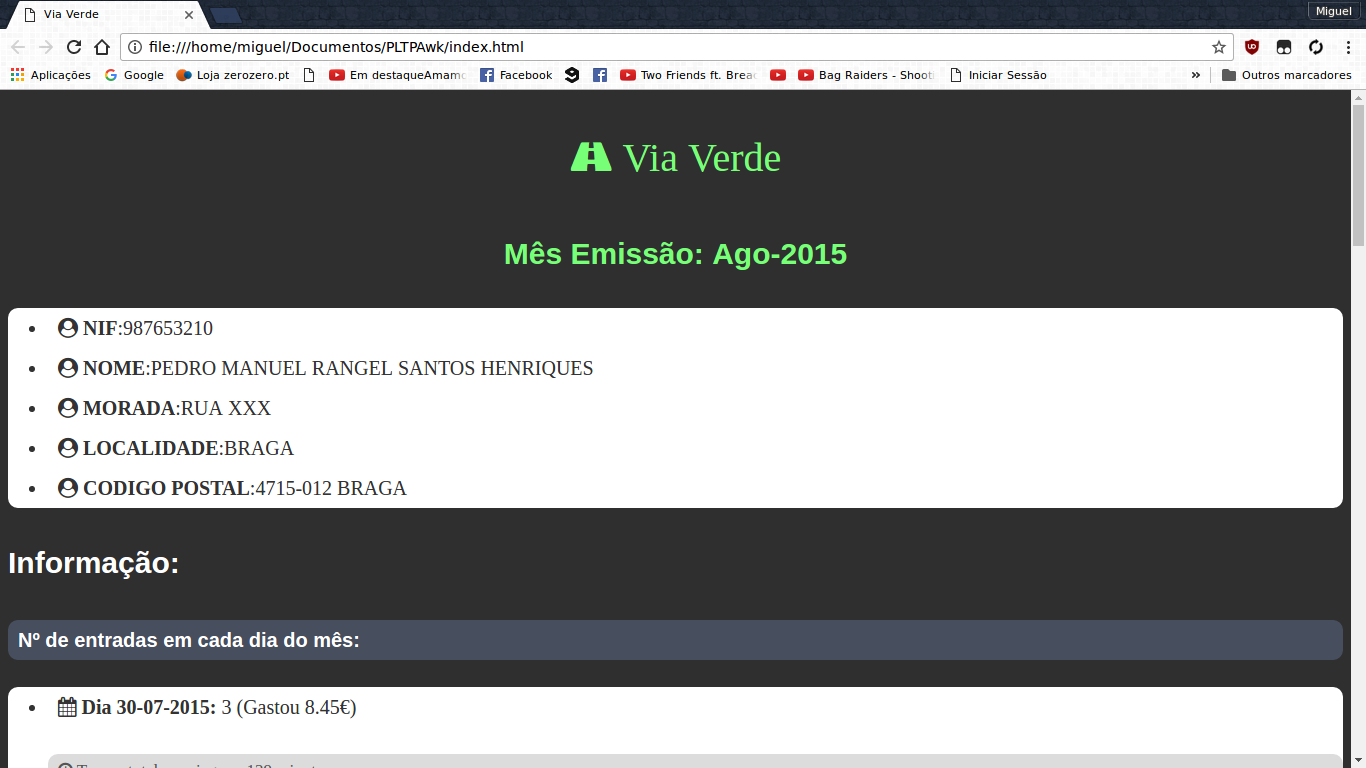
\includegraphics[scale=0.35]{out1.png}\par
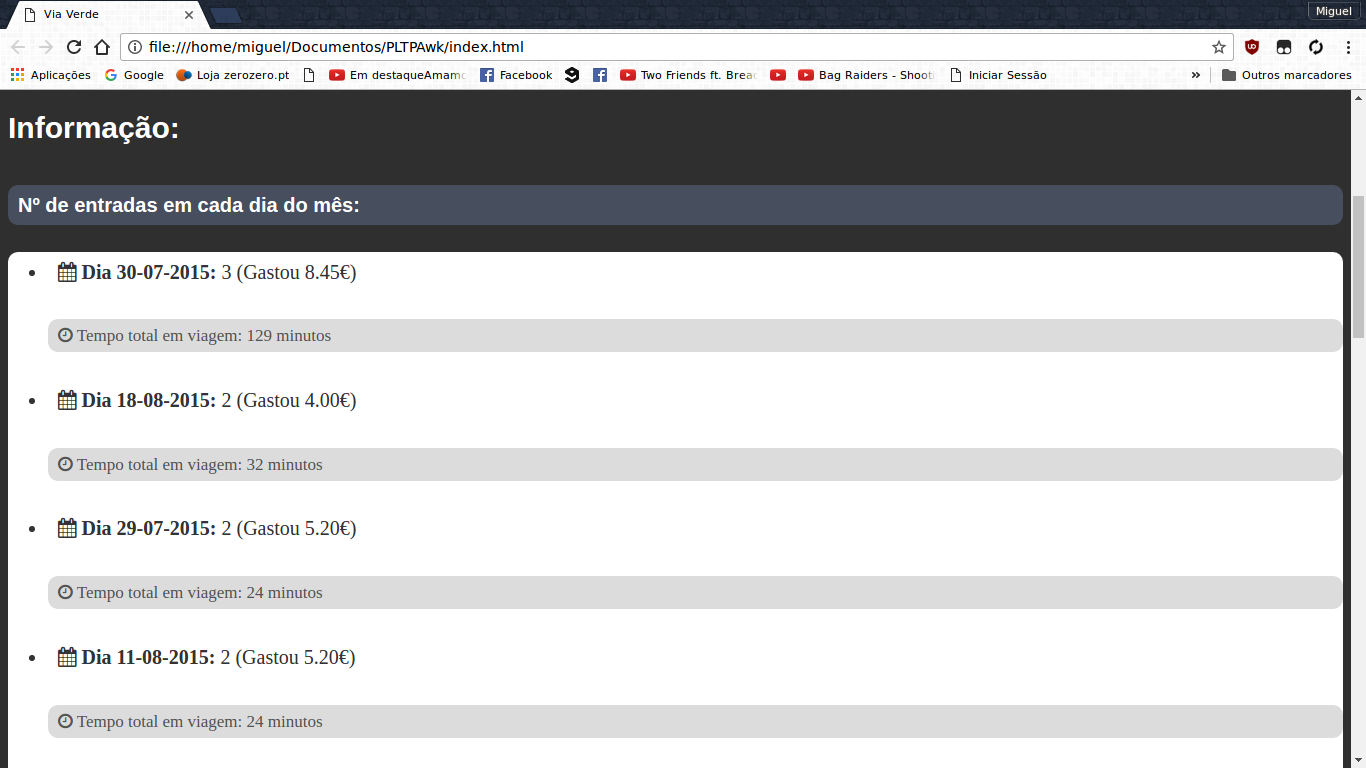
\includegraphics[scale=0.35]{out2.png}\par
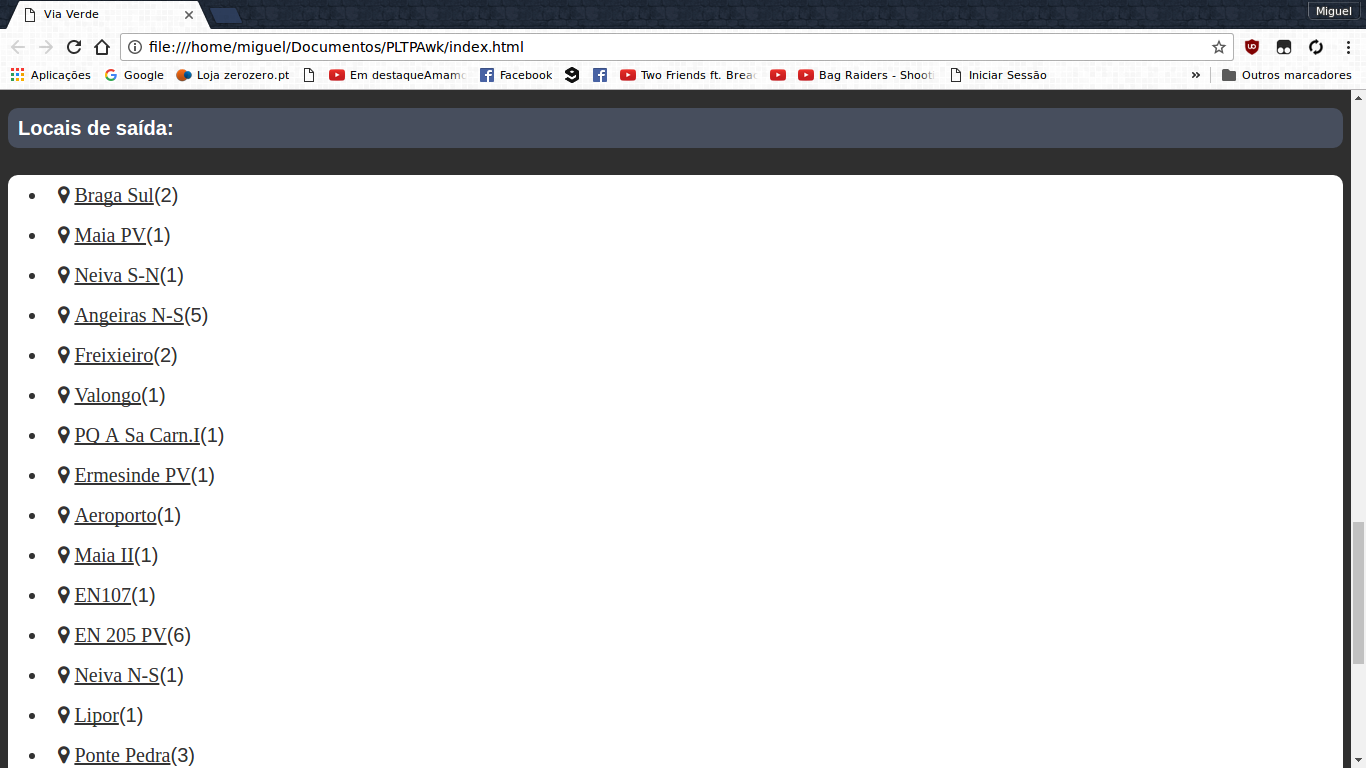
\includegraphics[scale=0.35]{out3.png}\par
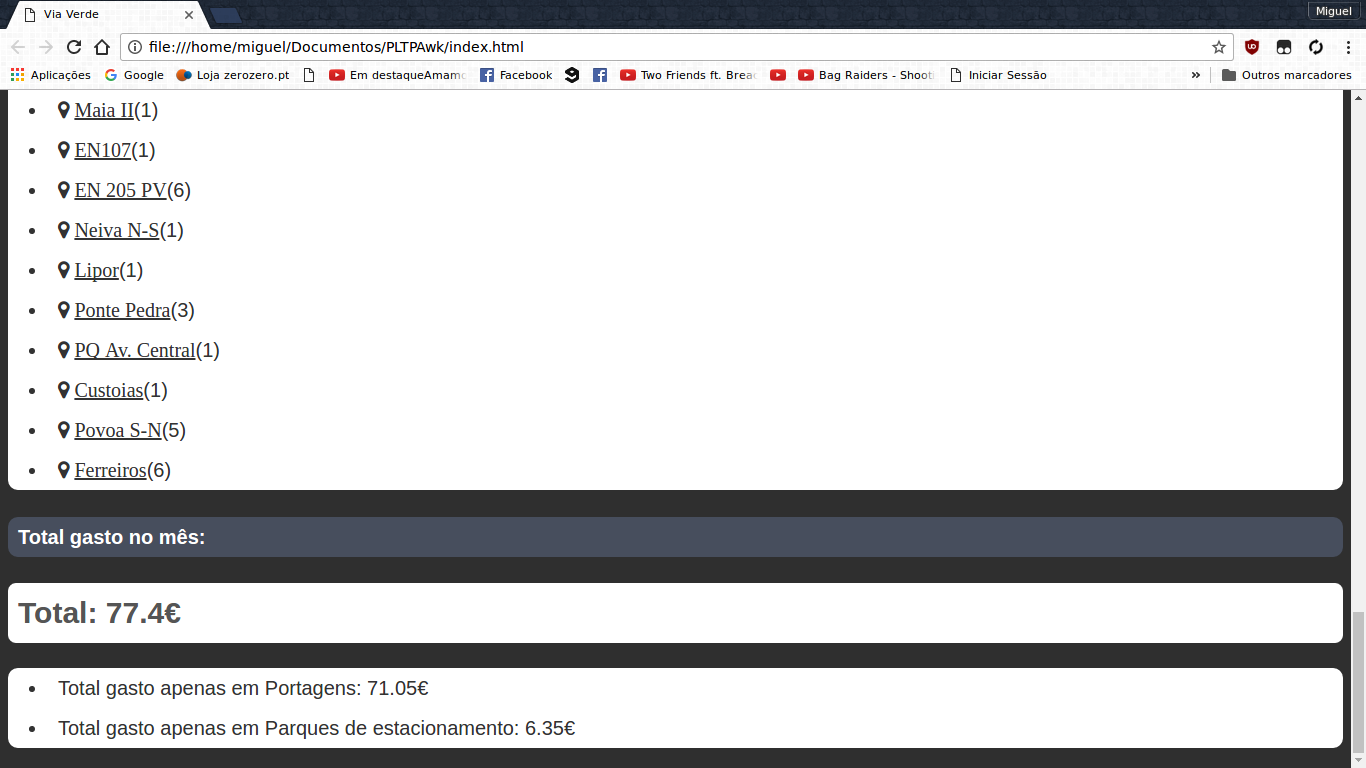
\includegraphics[scale=0.35]{out4.png}

\subsection{Exemplo da tab que abre quando se clica no local Ferreiros}

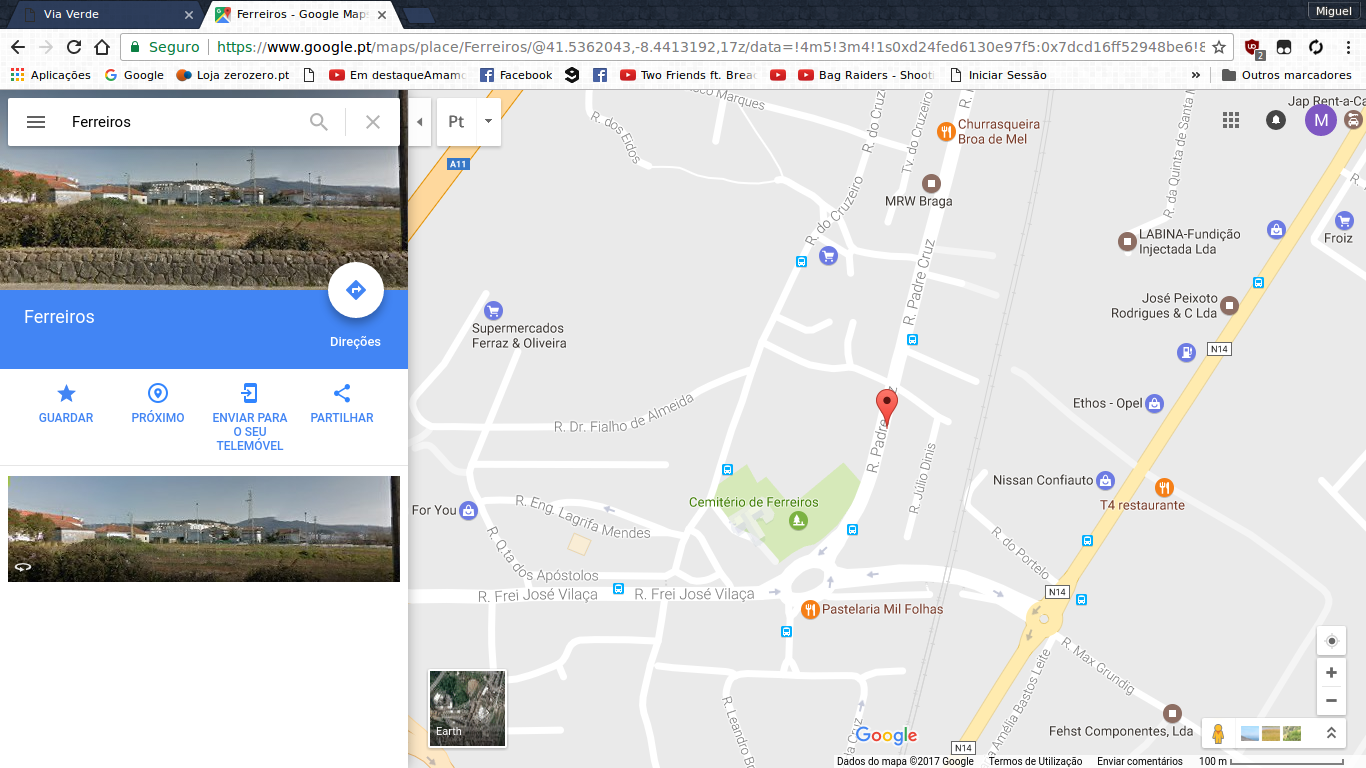
\includegraphics[scale=0.35]{maps.png}\par

\subsection{Exemplo da lista que abre quando se clica numa data}

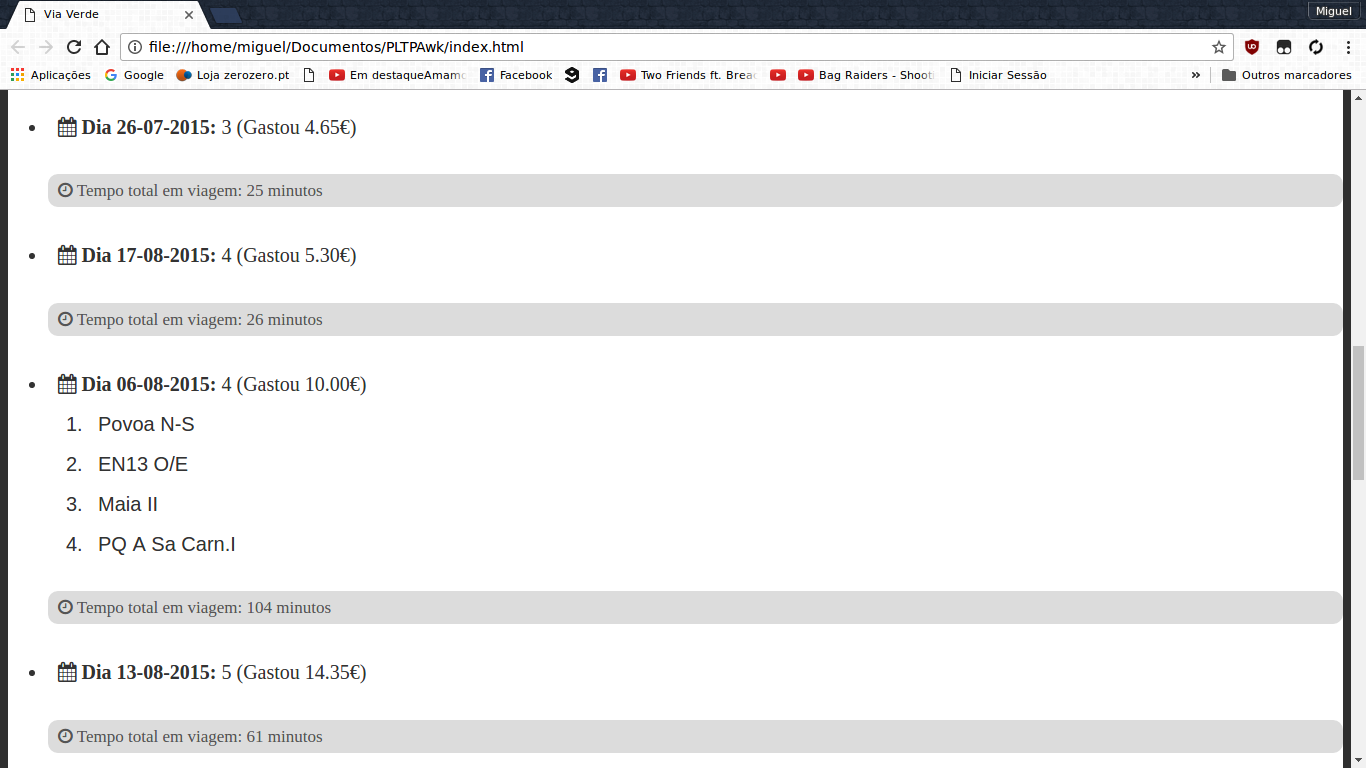
\includegraphics[scale=0.35]{out5.png}\par

\chapter{Conclusão} \label{concl}
Foi possível, 
através do uso da liguagem de programação AWK e do uso de ferramentas html, realizar com sucesso os 
requisitos pedidos neste trabalho prático assim como demostrar outras funcionalidades importantes e úteis para a 
recolha e apresentação de informação neste trabalho.
Para além dos requisitos necessários, calcular o número de entradas do utente em cada dia do mês, obter a 
lista de locais de saída utlizados durante o mês
retirar o valor total pago no final do mês e o valor total relativo apenas ao estacionamento em parques, 
foi possível apresentar mais informação detalhada, tais como
o total gasto em cada dia, a duração total de viagens e visualização dos locais de saída num mapa para melhor orientação.\par

Com o uso de expressões regulares GAWK foi possível encontrar a informação específica do ficheiro xml, logo possibilitando 
retirar essa mesma e guardá-la em arrays associativos
para posterior apresentação em formato html. Este foi utilizado como formato de apresentação visto que apresenta a informação 
necessária num formato conciso e elegante, 
apesar de ser mais complexo do que usar o standard output. Para melhorar a desposição da informação e simplicidade desta foi 
utilizado a font-awesome visto que esta permitiria criar 
icons relativos a cada linha para melhor compreensão e para apelar ao utilizador, permitindo uma maior fluidez na procura 
dos conteúdos .\par
O uso das expressões regulares através da linguagem de programação AWK e de ferramentas html permitiu, em termos de processamento 
de texto e divulgação, gerar código simples e curto,
de fácil compreensão e com a capacidade necessária para retirar, armazenar e apresentar informação importante e relativa ao projeto. 
Com isto dito, existem ainda capacidades extra
por explorar para continuar a desenvolver o projeto, tais como, a disponibilização de um trajeto feito pelo utente num determinado dia. 
Logo apesar de completar os requisitos necessários
com as capacidades da linguagem AWK, é possível encontrar novas maneiras de utilizar a informação disposta, de forma a proporcionar maior 
utilidade ao utentes e gestores.
   


\appendix 
\chapter{Código do Programa}

Lista-se a seguir o código  do programa  que foi desenvolvido.

\lstinputlisting{procViaverde}%input de um ficheiro

\bibliographystyle{alpha}
\bibliography{relprojLayout}



\end{document}
